%%% Folie
{
\small

\begin{frame}{Ausgangslage}
    \parbox{\linewidth}{
        In seiner Standardkonfiguration ist der Raspberry Pi nur begrenzt für größere
        IoT-Anwendungsfälle geeignet, da das mitgelieferte Raspbian-Betriebssystem
        hierfür nicht ausgelegt ist. Dies liegt daran, dass der Raspberry Pi
        hauptsächlich als einfaches Lern- und Experimentiergerät in der Tradition
        früherer Heimcomputer entworfen wurde. Jedoch lässt sich das Betriebssystem
        sehr leicht anpassen oder durch ein maßgeschneidertes Embedded Linux ersetzen.
    }

    \medskip

    \begin{columns}[b,onlytextwidth]
        \column{.48\textwidth}
        \begin{center}
            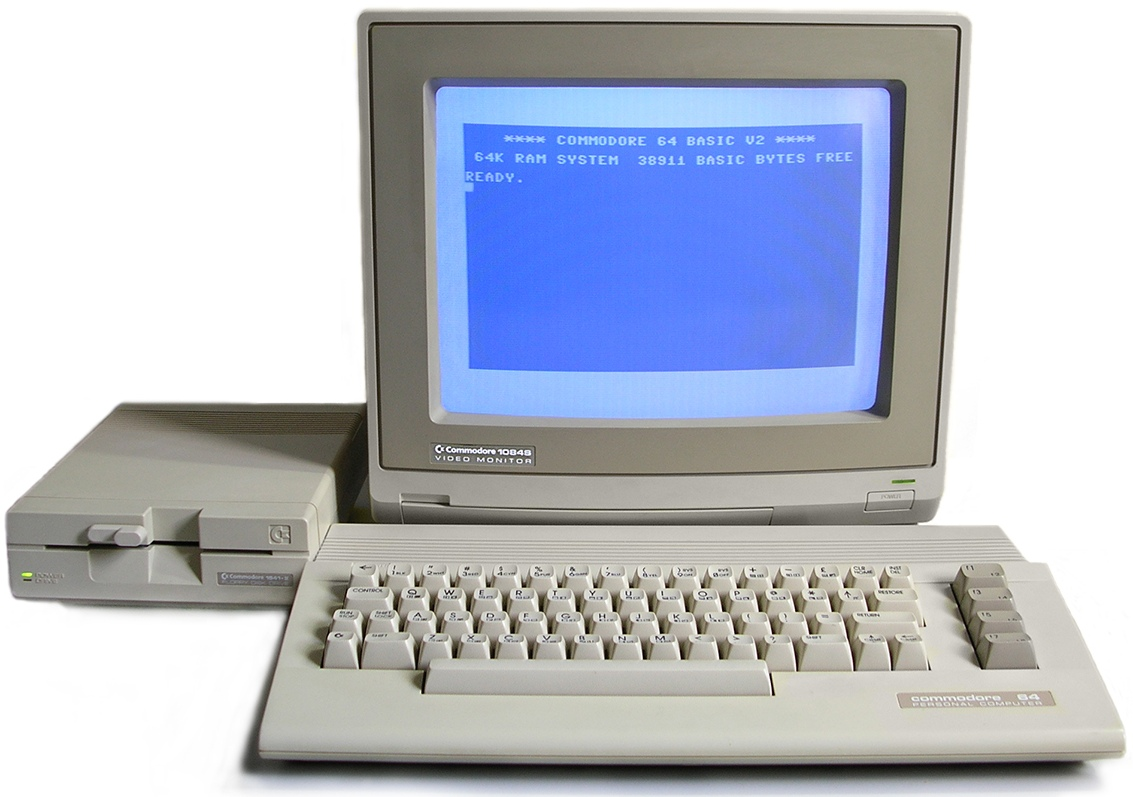
\includegraphics[width=.9\textwidth]{img/c64}
        \end{center}
        \parbox{\linewidth}{
            \footnotesize
            \textbf{Commodore 64:}
            Beispiel für einen weit verbreiteten Heimcomputer der 1980er-Jahre
            mit eingebautem BASIC-Interpreter
        }

        \column{.48\textwidth}
        \begin{center}
            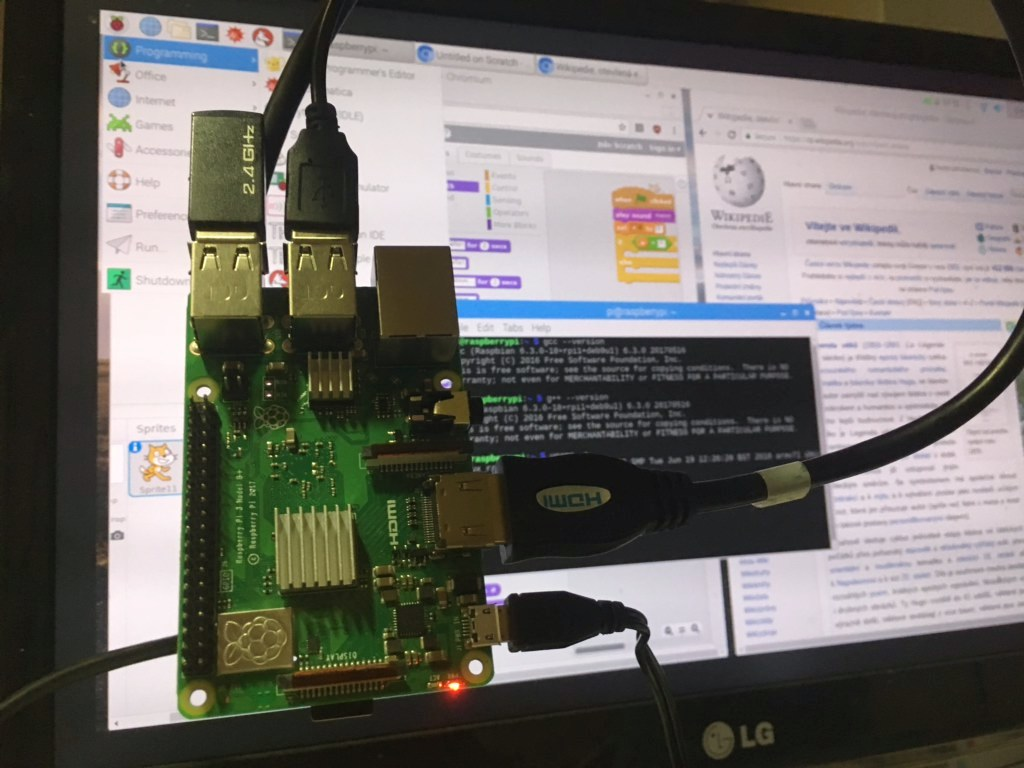
\includegraphics[width=.85\textwidth]{img/raspi}
        \end{center}
        \parbox{\linewidth}{
            \footnotesize
            \textbf{Rasbperry Pi:} Modermer Versuch, einen Computer zum
            Experimentieren und Programmieren Lernen zu bauen
        }
    \end{columns}
\end{frame}
}

%%% Folie
\begin{frame}{Lernziele}
    \begin{block}{Bestandteile eines Linux-Systems}
        \begin{itemize}
            \item Den typischen Aufbau eines Linux-Systems beschreiben können
            \item Das Partitionsschema des Raspberry Pi kennen und verstehen
            \item Den Filesystem Hierarchy Standard kennen und verstehen
            \item Die Benutzer- und Rechteverwaltung von Linux nutzen können
            \item Den Bootvorgang des Raspberry Pi vollständig erklären können
            \item Die Aufgaben und Funktionsweise des Init-Systems erklären können
            \item Eigene Python-Programme installieren und automatisch starten können
        \end{itemize}
    \end{block}

    \begin{block}{Erstellung eigener Linux-Systeme}
        \begin{itemize}
            \item Die Vorgehensweise beim Bau eigener Images kennen und verstehen
            \item Ein geeignetes Toolkit zum Bau von Linux-Systemen auswählen können
            \item Die groben Schritte zur Nutzung der Toolkits beschreiben können
            \item Eigene Programme in die selbst erstellten Images integrieren können
        \end{itemize}
    \end{block}
\end{frame}

%%% Folie
\begin{frame}{Inhaltsübersicht}
    \tikzset{
        MyTitle/.style={
            align=left,
            text=blue!65!purple,    % 65% blue, 35% purple
            anchor=north west,
            font=\large,
        },
        MyNode1/.style={
            below=2pt,
            align=left,
            anchor=north west,
            font=\footnotesize
        },
        MyNode2/.style={
            above=2pt,
            align=left,
            anchor=south west,
            font=\footnotesize
        },
        MyNumber/.style={
            text=white,
            font=\scriptsize
        }
    }

    % Vgl. https://tex.stackexchange.com/a/18201
    \pgfdeclarelayer{bg}
    \pgfsetlayers{bg, main}

    \begin{columns}
        \column{\dimexpr\paperwidth-1.4cm}
        \begin{tikzpicture}
            % Bestandteile eines Linux-Systems
            \node[MyTitle] at (0,0) {Bestandteile eines Linux-Systems};
            \filldraw[fill=darkred]
                ( 0,-0.6) circle(4pt) node(pi-1){} node[MyNumber]{1}  node[MyNode1]{Der grundsätzliche Aufbau \\ eines Linux-Systems}
                ( 4,-0.6) circle(4pt) node(pi-2){} node[MyNumber]{2}  node[MyNode1]{Der Linux Filesystem \\ Hierarchy Standard}
                ( 8,-0.6) circle(4pt) node(pi-3){} node[MyNumber]{3}  node[MyNode1]{Benutzer- und Rechte- \\ verwaltung unter Linux};
            \filldraw[fill=gray!50]
                (11,-0.6) circle(4pt) node(pi-tr){}
                (11,-2.6) circle(4pt) node(pi-br){};
            \filldraw[fill=darkred]
                ( 8,-2.6) circle(4pt) node(pi-4){} node[MyNumber]{4}  node[MyNode2]{Der Bootvorgang des \\ Raspberry Pi im Detail}
                ( 4,-2.6) circle(4pt) node(pi-5){} node[MyNumber]{5}  node[MyNode2]{Konfiguration des \\ Linux-Startvorgangs}
                ( 0,-2.6) circle(4pt) node(pi-6){} node[MyNumber]{6}  node[MyNode2]{Fallbeispiel: Automatischer \\ Start eines Pythonprogramms};

            % Erstellung eigener Linux-Systeme
            \node[MyTitle] at (0,-3.4) {Erstellung eigener Linux-Systeme};
            \filldraw[fill=darkred]
                ( 0,-4.0) circle(4pt) node(mk-1){} node[MyNumber]{7}  node[MyNode1]{Generelles Vorgehen beim \\ Bau eines Firmware-Images}
                ( 4,-4.0) circle(4pt) node(mk-2){} node[MyNumber]{8}  node[MyNode1]{Vergleich verschiedener \\ Baukästen für Linux}
                ( 8,-4.0) circle(4pt) node(mk-3){} node[MyNumber]{9}  node[MyNode1]{Linux-Images bauen \\ mit pi-gen};
            \filldraw[fill=gray!50]
                (11,-4.0) circle(4pt) node(mk-tr){}
                (11,-6.0) circle(4pt) node(mk-br){};
            \filldraw[fill=darkred]
                ( 8,-6.0) circle(4pt) node(mk-4){} node[MyNumber]{10} node[MyNode2]{Linux-Images bauen \\ mit Buildroot}
                ( 4,-6.0) circle(4pt) node(mk-5){} node[MyNumber]{11} node[MyNode2]{Fazit und Ausblick};
            \filldraw[fill=gray!50]
                ( 0,-6.0) circle(4pt) node(mk-6){};

            % Verbindungslinien
            \begin{pgfonlayer}{bg}
                \draw (pi-1) -- (pi-2) -- (pi-3) -- (pi-tr) -- (pi-br) -- (pi-4) -- (pi-5) -- (pi-6);
                \draw[gray, densely dashed] (pi-6) -- (mk-1);
                \draw (mk-1) -- (mk-2) -- (mk-3) -- (mk-tr) -- (mk-br) -- (mk-4) -- (mk-5) -- (mk-6);
            \end{pgfonlayer}
        \end{tikzpicture}
    \end{columns}
\end{frame}

%-------------------------------------------------------------------------------
\section{Bestandteile eines Linux-Systems}
%-------------------------------------------------------------------------------

%%% Folie
\begin{frame}{Beispiele für Linux-basierte Betriebssysteme}
    \parbox{\linewidth}{
        \footnotesize
        Linux bezeichnet im engeren Sinne kein Betriebssystem sondern nur einen
        Kernel, der die Grundlage für viele Betriebssysteme (Linux-Distributionen)
        auf den unterschiedlichsten Computersystemen bildet. Linux kann dabei auf
        nahezu jeder Hardware betrieben werden.
        \medskip
    }

    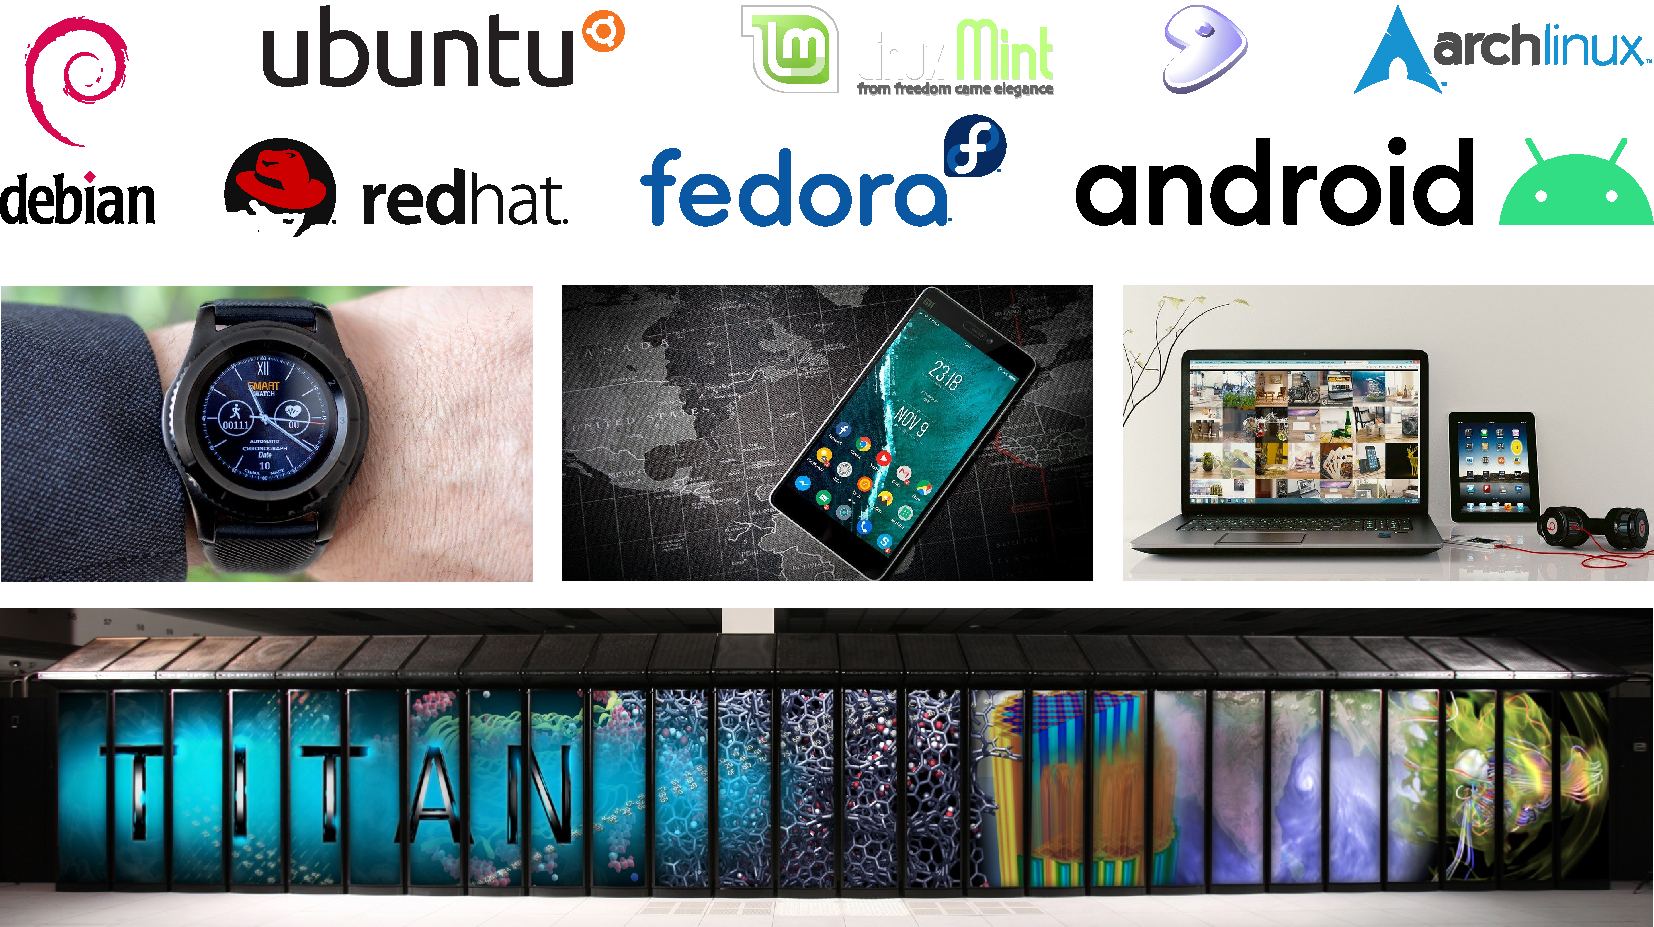
\includegraphics[width=\textwidth]{img/linux-beispiele}
\end{frame}

%%% Folie
{
\footnotesize
\setlength{\leftmargini}{1.2em}

\begin{frame}{Kernel vs. Userland}
    \parbox{\linewidth}{
        Linux-basierte Betriebssysteme setzen sich immer aus dem \textbf{Kernel}
        und dem \textbf{Userland} zusammen. Der Kernel beinhaltet dabei lediglich
        die Grundfunktionen für Hardwarezugriffe, Multitasking, Speicherverwaltung
        usw. Alle anderen Teile des Betriebssystems sind Bestandteil des Userlands
        und können somit stark variieren.
    }

    \vfill

    {
        \scriptsize

        \begin{columns}[T,onlytextwidth]
            \column{.49\textwidth}
            \begin{itemize}
                \justifying

                \item \textbf{Bibliotheken:} Von den installierten Programmen
                benötigte Quellcode-Bibliotheken mit gemeinsamen Funktionen.
                Zum Beispiel \texttt{libc} oder \texttt{libgtk}.

                \item \textbf{Systemdienste:} Hintergrundjobs und Hilfsprogramme des
                Betriebssystems. Zum Beispiel NTP-Daemon, Druckerspooler oder die
                Shell bzw. grafische Desktopumgebung.

                \item \textbf{Anwendungen:} Nicht direkt zum Betriebssystem gehörende,
                jedoch zur Nutzung durch die Anwender*innen vorgesehene Programme, wie
                zum Beispiel Webbrowser oder Media Player.
            \end{itemize}

            \column{.49\textwidth}
            \begin{itemize}
                \justifying

                \item \textbf{Variable Daten:} Während dem regulären Systembetrieb
                anfallende Verwaltungsdaten, wie Systemprotokolle, temporäre Dateien
                oder zwischengespeicherte Druckaufträge.

                \item \textbf{Benutzerdaten:} In der Hoheit der Benutzer*innen liegende
                Dateien, wie zum Beispiel Bilder oder Dokumente.
            \end{itemize}
        \end{columns}
    }

    \vfill
    $\Rightarrow$ \textbf{GNU/Linux:} Linux-Kernel mit GNU-Userland (plus weiteren Bestandteilen) \\
    $\Rightarrow$ \textbf{Android:} Linux-Kernel mit nahezu komplett in Java entwickeltem Userland

    \vfill
    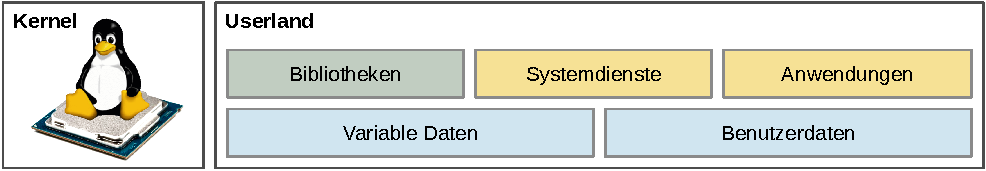
\includegraphics[width=\textwidth]{img/linux-bestandteile}
\end{frame}
}


%%% Folie
\begin{frame}{Partitionen und Dateisysteme auf dem Raspberry Pi}
    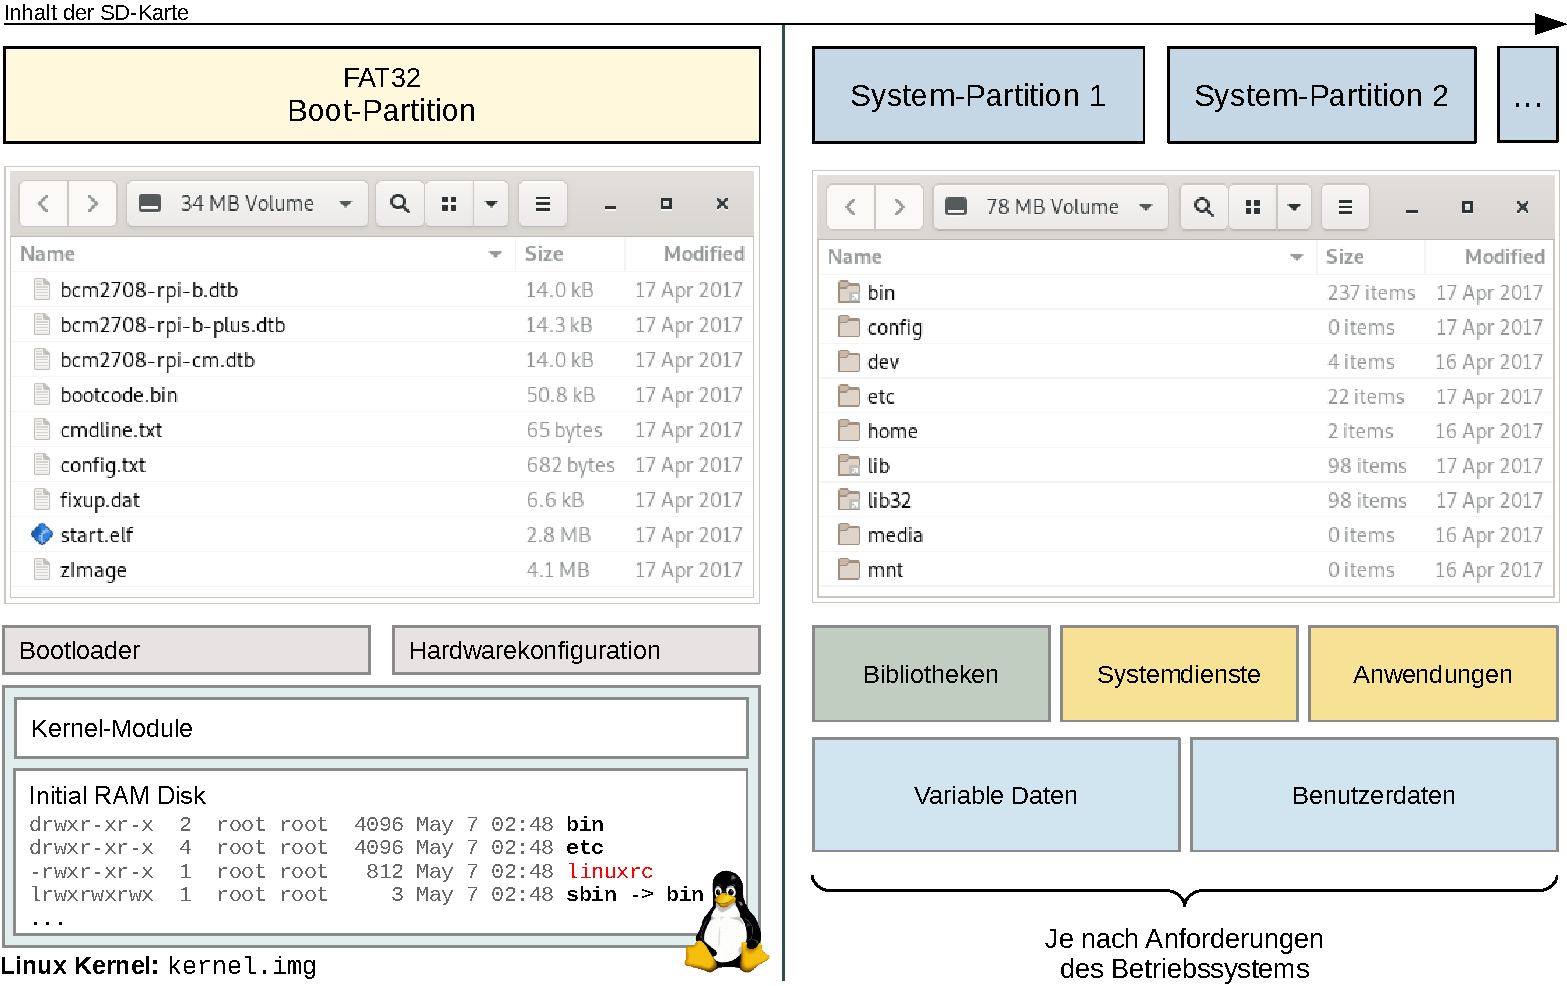
\includegraphics[width=\textwidth]{img/pi-partitionen}
\end{frame}

%%% Folie
{
\footnotesize

\begin{frame}[allowframebreaks]{Der Linux Filesystem Hierarchy Standard}
    \begin{center}
        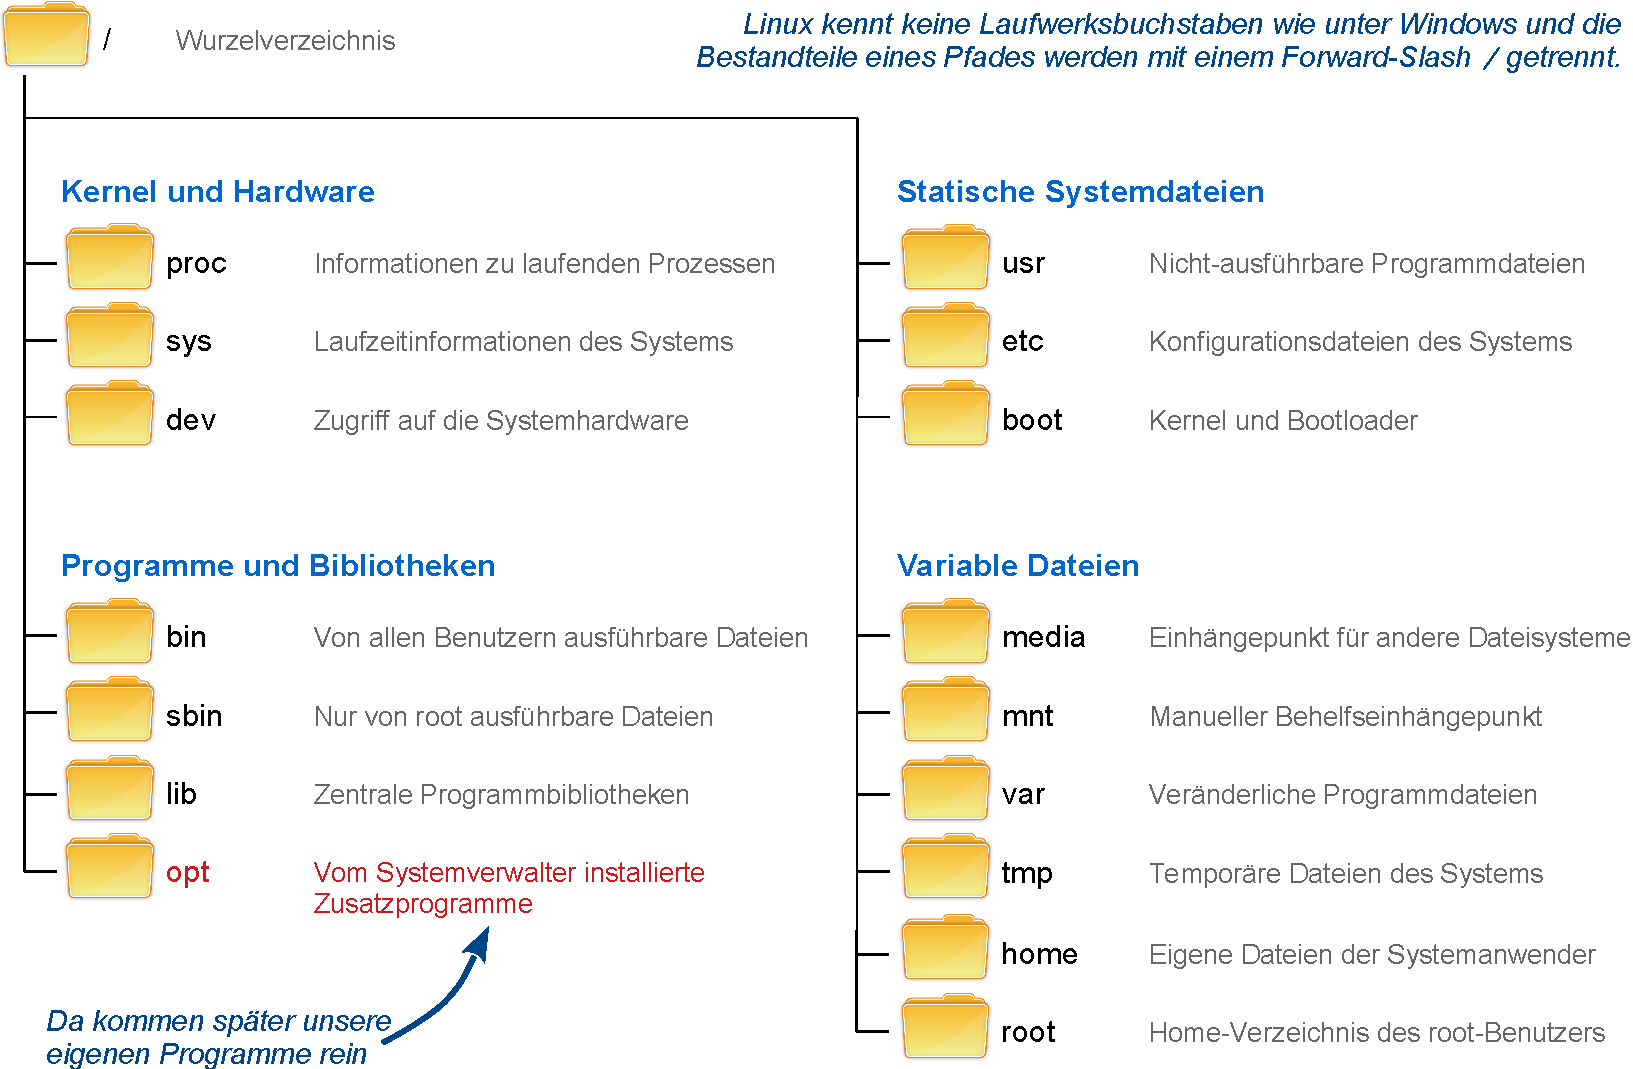
\includegraphics[width=\textwidth]{img/fhs-verzeichnisse}
    \end{center}

    \framebreak

    \begin{columns}[T]
        \column{.8\textwidth}
        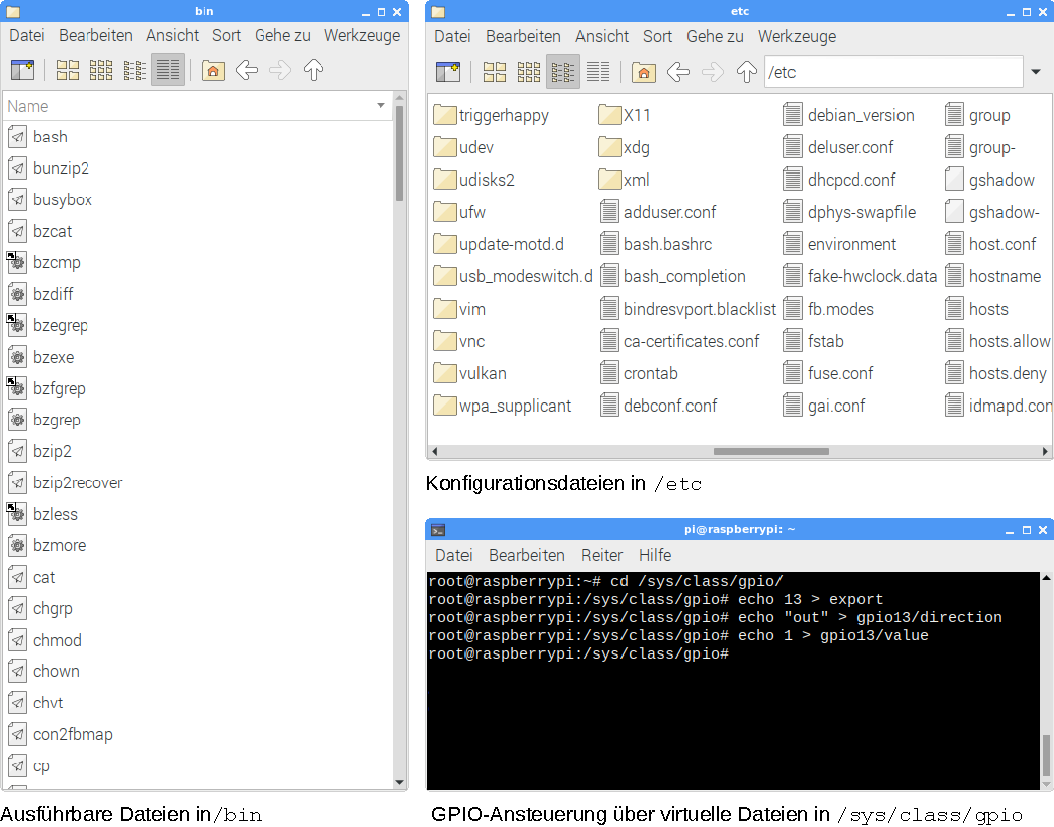
\includegraphics[width=\textwidth]{img/fhs-beispiele}

        \column{.3\textwidth}
        \parbox{\linewidth}{
            Aufgrund der konzeptionellen Nähe zu Unix ist unter Linux fast alles
            eine Datei. Die Konfiguration des Systems erfolgt deshalb genau so
            durch Editieren von Konfigurationsdateien, wie der Zugriff auf einen
            Hardwarebaustein nicht viel mehr als das Lesen und Schreiben virtueller
            Dateien erfordert.
        }
    \end{columns}
\end{frame}
}

%%% Folie
{
\footnotesize

\begin{frame}[allowframebreaks]{Benutzer- und Rechteverwaltung unter Linux}
    \begin{columns}[onlytextwidth]
        \column{.55\textwidth}
        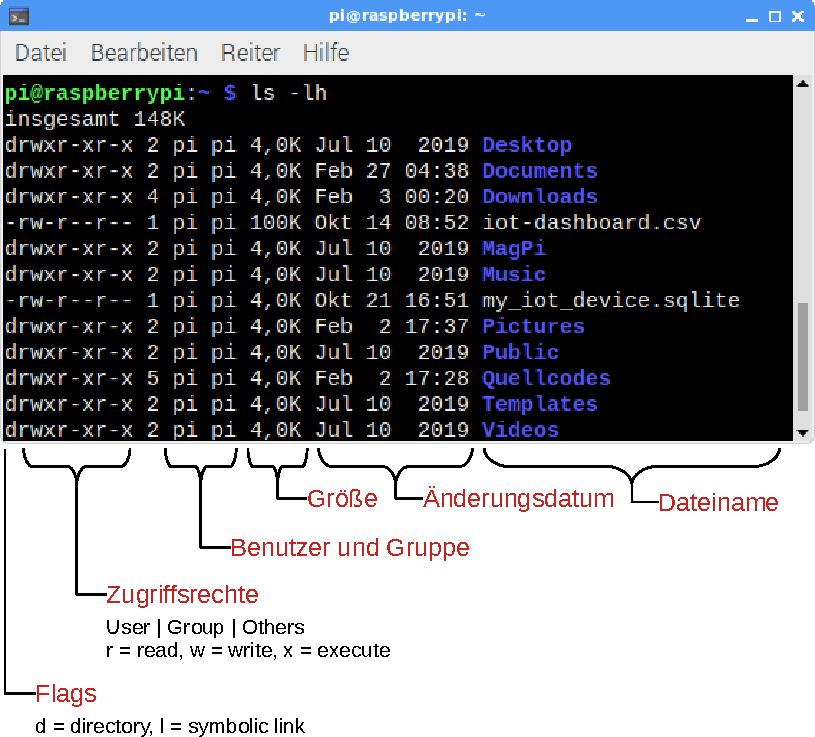
\includegraphics[width=\textwidth]{img/rechte-dateizugriff}

        \column{.4\textwidth}
        \parbox{\linewidth}{
            Alle Einträge im Dateisystem sind immer genau einem Benutzerkonto
            und einer Benutzergruppe zugeordnet. Zusätzlich besitzen sie ein
            Bit-Feld mit Zugriffsrechten für

            \begin{itemize}
                \item den Benutzer,
                \item die Benutzergruppe,
                \item den Rest der Welt.
            \end{itemize}

            Über dieses Feld wird gesteuert, ob Lese-, Schreib- oder ausführende
            Zugriffe erlaubt sind.

            \medskip

            \glqq{}Ausführen\grqq{} bedeutet bei einer Datei, diese als Programm
            zu starten. Bei einem Verzeichnis bedeutet es, die Inhalte des
            Verzeichnisses zu sehen.

            \medskip

            Die Berechtigungsprüfung wird immer mit dem Benutzerkonto durchgeführt,
            unter dessen Namen ein zugreifendes Programm läuft.
        }
    \end{columns}

    \medskip
    \textbf{Wichtige Befehle}

    \begin{columns}[onlytextwidth]
        \column{.33\textwidth}
        \texttt{chown} \\ Benutzer/Gruppe ändern

        \column{.33\textwidth}
        \texttt{chmod} \\ Zugriffsrechte ändern

        \column{.33\textwidth}
        \texttt{sudo} \\ Programm unter anderem Benutzer starten
    \end{columns}

    %%
    \framebreak

    \begin{center}
        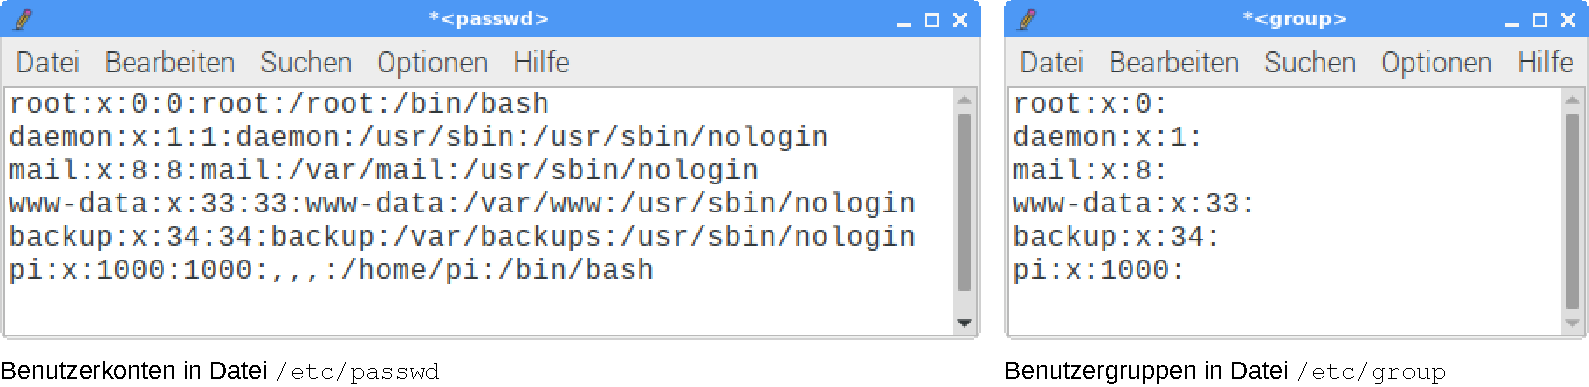
\includegraphics[width=\textwidth]{img/rechte-konfiguration}
    \end{center}

    \parbox{\linewidth}{
        Die Benutzerkonten und Benutzergruppen sind in den Dateien
        \texttt{/etc/passwd} und \texttt{/etc/group} definiert. Jeder
        Benutzer bzw. jede Benutzergruppe bekommt hier eine numerische ID
        zugewiesen, die sehr oft nach folgendem Schema vergeben wird:
    }

    \medskip

    {
        \scriptsize
        \renewcommand{\arraystretch}{1.4}
        \setlength{\tabcolsep}{0em}

        \begin{tabularx}{\textwidth}{p{.11\textwidth} p{.2\textwidth} X}
            \hline
            \textbf{UID/GID} & \textbf{Bezeichnung} & \textbf{Bedeutung} \\
            \hline

            0 & Benutzer \texttt{root} & Superuser mit maximalen Berechtigungen \\
            1 -- 999 & Systembenutzer & Technische Benutzer zur Ausführung der Systemdienste \\
            $\geq$ 1000 & Interaktive Benutzer & Menschliche Benutzer mit Login-Möglichkeit \\
            \hline
        \end{tabularx}
    }

    \medskip
    \textbf{Wichtige Befehle}
    {
        \setlength{\leftmargini}{1.2em}
        \begin{columns}[T, onlytextwidth]
            \column{.5\textwidth}
            \begin{itemize}
                \item \texttt{adduser}: Neues Benutzerkonto anlegen
                \item \texttt{deluser}: Benutzerkonto löschen
                \item \texttt{usermod}: Benutzerkonte bearbeiten
            \end{itemize}

            \column{.5\textwidth}
            \begin{itemize}
                \item \texttt{passwd}: Benutzerpasswort ändern
                \item \texttt{groupadd}: Neue Benutzergruppe anlegen
                \item \texttt{delgroup}: Benutzergruppe löschen
            \end{itemize}
        \end{columns}
    }
\end{frame}
}

%%% Folie
\begin{frame}{Der Bootvorgang des Raspberry Pi im Detail}
    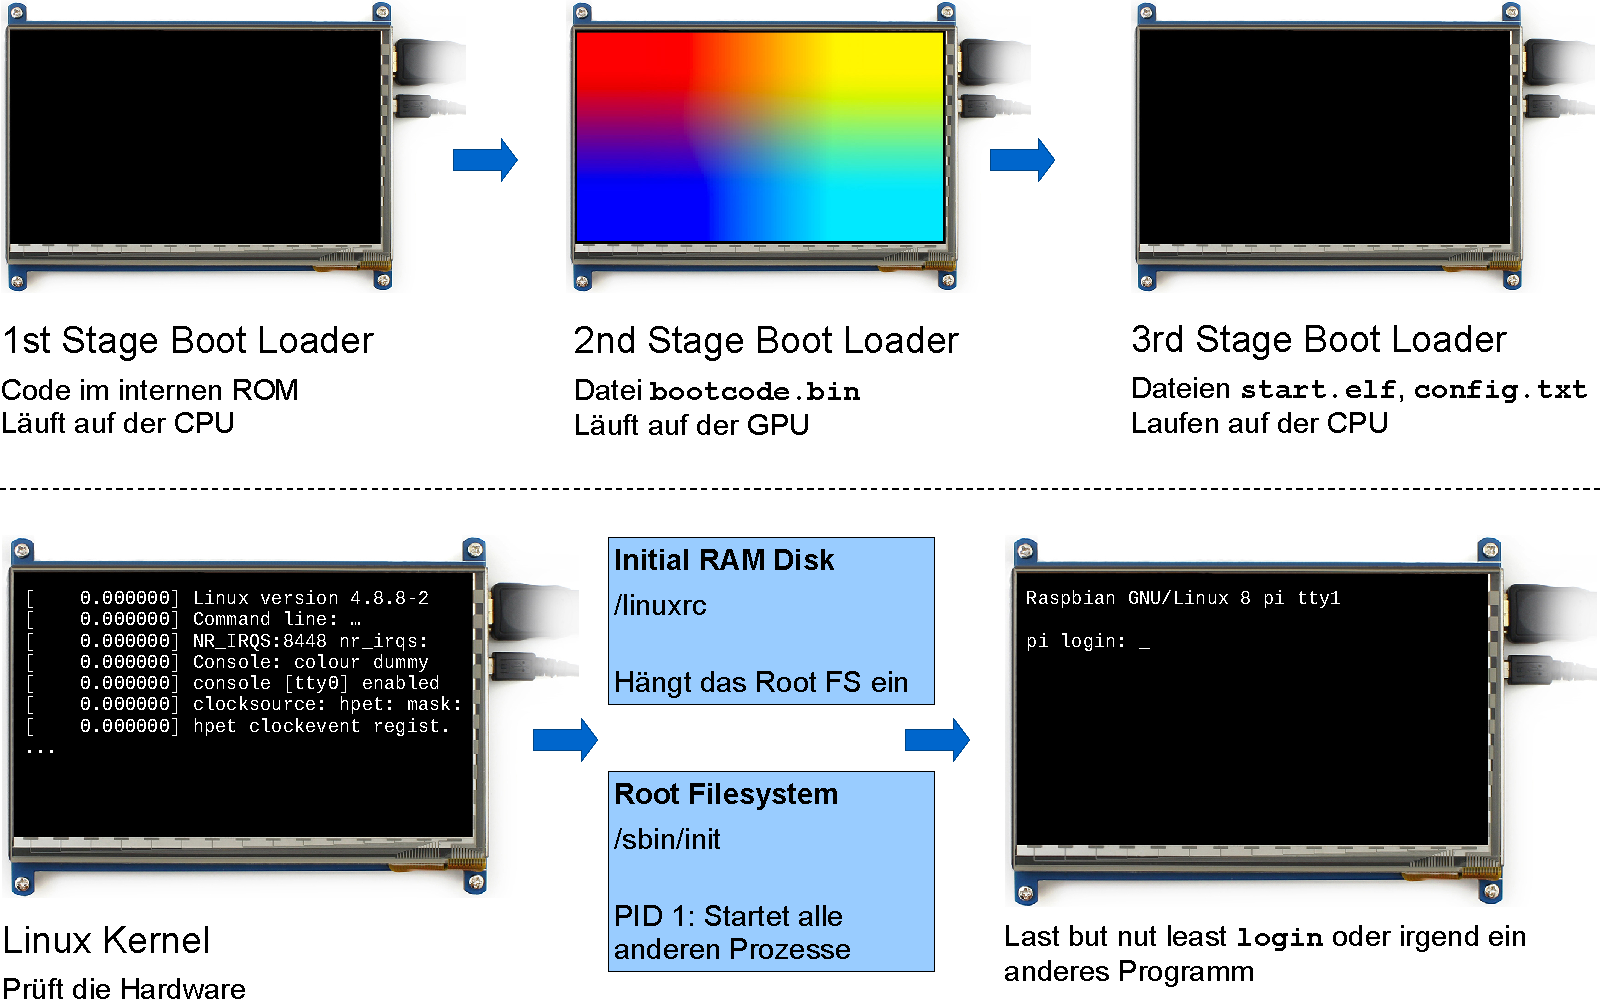
\includegraphics[width=\textwidth]{img/pi-bootvorgang}
\end{frame}

%%% Folie
{
\footnotesize

\begin{frame}[allowframebreaks]{Automatischer Start der Systemdienste}
    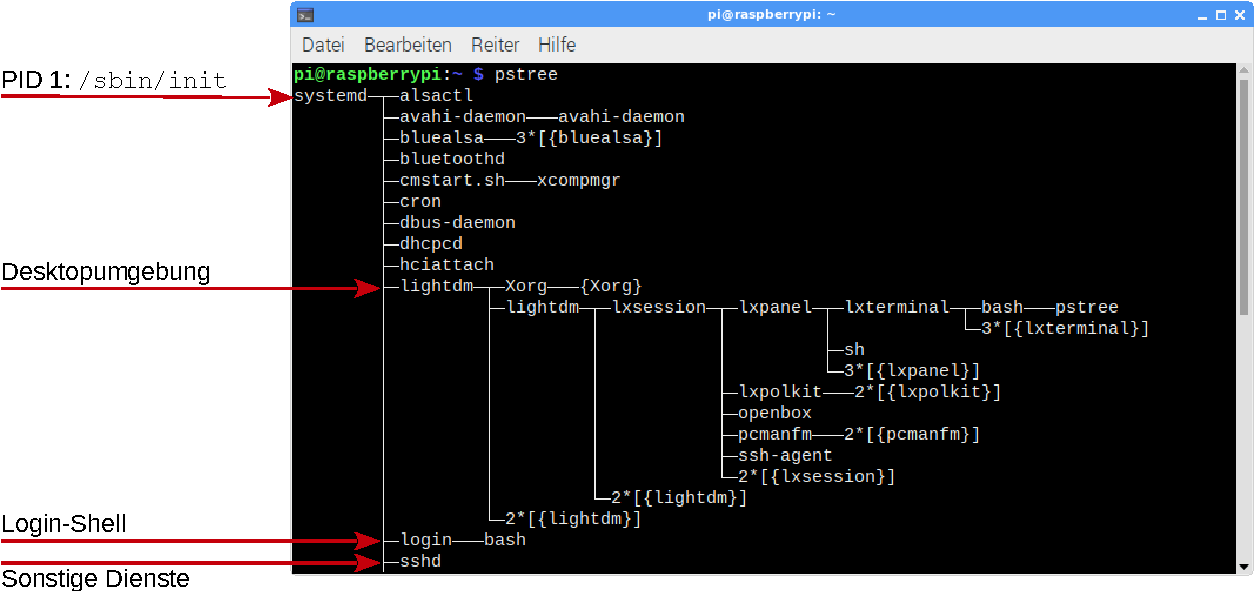
\includegraphics[width=\textwidth]{img/pid1-pstree}
    \medskip

    \parbox{\linewidth}{
        Nachdem der Kernel die Hardware geprüft und initialisiert hat, wird die
        Verarbeitung zunächst an das Programm \texttt{/linuxrc} in der Initial
        RAM Disk und von diesem an das Programm \texttt{/sbin/init} im Root
        Filesystem übergeben. Dieses erhält die Prozess ID 1 und ist dafür
        verantwortlich, alle anderen Systemdienste zu starten. Es handelt sich
        dabei um das einzige Programm unter Linux, das niemals beendet werden
        darf, da sonst das System mit einer Kernel Panic abstürzt.
    }

    %%
    \framebreak

    \begin{block}{Variante 1: Einfaches Shellskript}
        \smallskip
        \parbox{\linewidth}{
            Im einfachsten Fall handelt es sich bei \texttt{/sbin/init} um ein
            einfaches Shellskript wie das folgende. Diese Variante könnte auf
            besonders schlanken, eingebetteten Systemen zum Einsatz kommen.
        }

        \lstinputlisting[language=bash]{code/init.sh}
    \end{block}

    %%
    \framebreak

    \begin{block}{Variante 2: SysV Init mit \texttt{/etc/inittab}}
        \smallskip
        \parbox{\linewidth}{
            Seit Unix System V wertet das Programm \texttt{/sbin/init} traditionell
            die Datei \texttt{/etc/inittab} aus, um die zu startenden Dienste zu
            ermitteln. Dort werden so genannte Run Level definiert, die das System
            beim Hoch- und Runterfahren erreichen kann. Zum Beispiel:
        }

        \vfill
        \begin{center}
            \scriptsize
            \begin{tabularx}{.8\textwidth}{X X}
                    \textbf{Run Level 0:} System herunterfahren &
                    \textbf{Run Level 2:} Mehrbenutzer-Modus \\

                    \textbf{Run Level 1:} Einzelbenutzer-Modus &
                    \textbf{Run Level 3:} Grafische Oberfläche \\
            \end{tabularx}
        \end{center}

        \vfill
        \parbox{\linewidth}{
            Am häufigsten kommt dieses Verfahren heutzutage noch in eingebetteten Systemen vor.
        }

        \vfill
        \lstinputlisting[language=bash]{code/inittab}
    \end{block}

    %%
    \framebreak

    \begin{block}{Variante 3: SystemD als moderner Standard}
        \smallskip
        \parbox{\linewidth}{
            Auf mittleren und großen Systemen hat sich inzwischen SystemD als Standard
            durchgesetzt. Vorteile sind, dass die zu startenden Dienste in einfachen
            Servicebeschreibungsdateien definiert werden und der gesamte Systemstart
            hochgradig parallelisiert abläuft. Debian bzw. Raspbian nutzen deshalb
            ebenfalls standardmäßig SystemD.
        }

        \bigskip
        \textbf{Vereinfachtes Beispiel: \texttt{/lib/systemd/system/sshd.service}}
        \lstinputlisting[language=Config]{code/sshd.service}

        \smallskip
        \textbf{Befehle zum Aktivieren und Starten des Services}
        \lstinputlisting[language=bash]{code/systemd-befehle.sh}
    \end{block}
\end{frame}
}

%%% Folie
{
\footnotesize

\begin{frame}{Fallbeispiel: Automatischer Start eines Pythonprogramms}
    \begin{columns}[onlytextwidth]
        \column{.58\textwidth}
        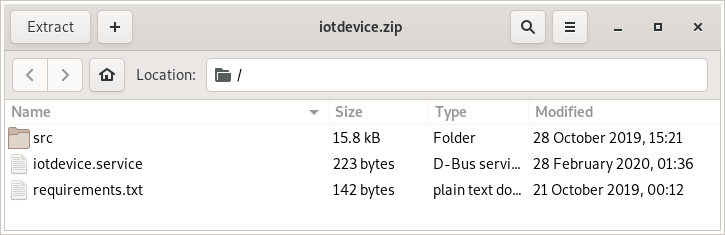
\includegraphics[width=\textwidth]{img/systemd-beispiel-zipfile}

        \column{.4\textwidth}
        \parbox{\linewidth}{
            Die Lösung zur Aufgabe \glqq{}Entwicklung eines IoT-Devices\grqq{}
            soll unter Raspbian systemweit installiert und beim Hochfahren
            automatisch gestartet werden. Die Desktop-Umgebung soll aus
            Performancegründen deaktiviert werden.
        }
    \end{columns}

    \bigskip
    \textbf{Inhalt der Datei \texttt{iotdevice.service}}
    \lstinputlisting[language=Config]{code/iotdevice.service}

    \medskip
    \textbf{Auszuführende Befehle}
    \vskip -.5em
    \begin{columns}[onlytextwidth]
        \column{.5\textwidth}
        \lstinputlisting[language=Config, linerange={1-8}]{code/iotdevice.install.sh}

        \column{.5\textwidth}
        \lstinputlisting[language=Config, linerange={9-16}, firstnumber=9]{code/iotdevice.install.sh}
    \end{columns}
\end{frame}
}

%-------------------------------------------------------------------------------
\section{Erstellung eigener Linux-Systeme}
%-------------------------------------------------------------------------------

%%% Folie
\begin{frame}{Generelles Vorgehen beim Bau eines Firmware-Images}
    \parbox{\linewidth}{
        Direkte Modifikationen im Raspbian-System bieten sich für kleine Projekte
        an, bei denen nur ein einzelner Raspberry Pi konfiguriert werden soll.
        Professioneller ist es jedoch, ein individuelles Linux-System auf einem
        Entwicklungsrechner zu bauen und dieses ohne manuelle Nacharbeiten auf
        beliebig vielen Raspberry Pis zu nutzen.
    }

    \vfill
    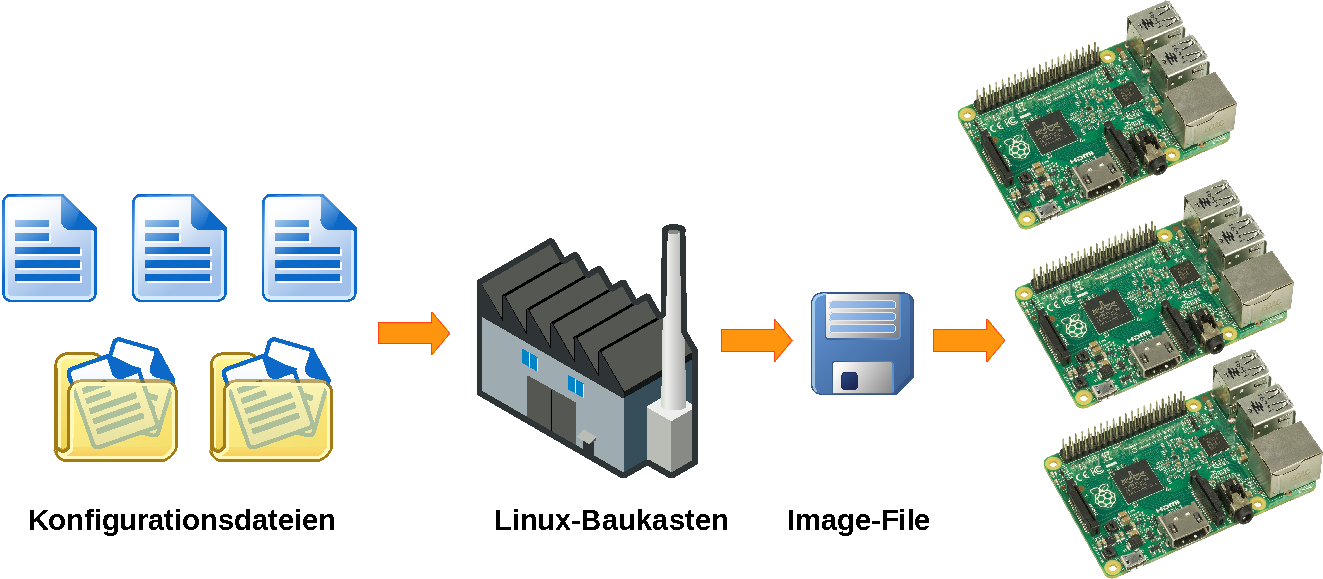
\includegraphics[width=\textwidth]{img/build-prinzip}
\end{frame}

%%% Folie
{
\scriptsize
\renewcommand{\arraystretch}{1.8}
\setlength{\tabcolsep}{0.5em}

\begin{frame}{Vergleich verschiedener Baukästen für Linux}
    \begin{columns}
        \column{\dimexpr\paperwidth-28pt}
        \parbox{\linewidth}{
            \footnotesize
            Die folgende Tabelle zeigt eine Übersicht häufig genutzter Baukastensysteme
            zur Erstellung individueller Linux-Systeme für Rasbperry Pi. Nicht dargestellt
            sind Yocto Linux, OpenWRT, Fedora CoreOS und viele weitere, in speziellen
            Bereichen weit verbreitete Distributionen.
        }

        \medskip

        \begin{tabular}{p{.21\textwidth} p{.25\textwidth} p{.25\textwidth} p{.25\textwidth}}
            &
            
\includegraphics[width=.10\textwidth]{img/Debian-OpenLogo1} &
            
\includegraphics[width=.08\textwidth]{img/Buildroot-logo} &
            
\includegraphics[width=.20\textwidth]{img/Ubuntu_logo} \\

            &
            \textbf{pi-gen} &
            \textbf{Buildroot} &
            \textbf{Ubuntu Core} \\
            \hline

            \textbf{Haupteinsatzgebiet} &
            Raspbian-Entwicklung & % pi-gen
            Eingebettete Systeme  & % Buildroot
            Desktop, Server, IoT \\ % Ubuntu Core

            \textbf{Funktionsweise} &
            Virtuelle Installation vorkompilierter Pakete in ein Image-File & % pi-gen
            Kompilieren aller Systembestandteile aus den Quellcodes & % Buildroot
            Virtuelle Installation vorkompilierter Pakete in ein Image-File \\ % Ubuntu Core

            \textbf{Paketformat} &
            DPKG & % pi-gen
            Quellcode + Makefiles & % Buildroot
            Snap \\ % Ubuntu Core

            \textbf{Anzahl Pakete} &
            ca. 30.000 & % pi-gen
            ca. 2.500  & % Buildroot
            ca. 5.000 \\ % Ubuntu Core

            \textbf{Customizbarkeit} &
            Hoch & % pi-gen
            Sehr hoch & % Buildroot
            Gering \\ % Ubuntu Core

            \textbf{OS-Upgrades} &
            Via APT-Paketverwaltung & % pi-gen
            Nicht direkt vorgesehen & % Buildroot
            Via Snapcraft \\ % Ubuntu Core

            \textbf{Init-System} &
            SystemD, andere möglich & % pi-gen
            Busybox, SysV oder SystemD & % Buildroot
            SyetemD \\ % Ubuntu Core

            \textbf{Userland} &
            GNU plus weitere  & % pi-gen
            Variabel, meist Busybox & % Buildroot
            GNU plus weitere \\ % Ubuntu Core

            \textbf{Anwendungsisoliation} &
            Möglich mit Docker oder LXC & % pi-gen
            Nicht direkt vorgesehen & % Buildroot
            Native unterstützt von Snap \\ % Ubuntu Core
        \end{tabular}
    \end{columns}
\end{frame}
}

%%% Folie
{
\small

\begin{frame}{Linux-Images bauen mit pi-gen}
    \href{https://github.com/RPi-Distro/pi-gen/blob/master/README.md}{\beamergotobutton{README-File}}

    \smallskip
    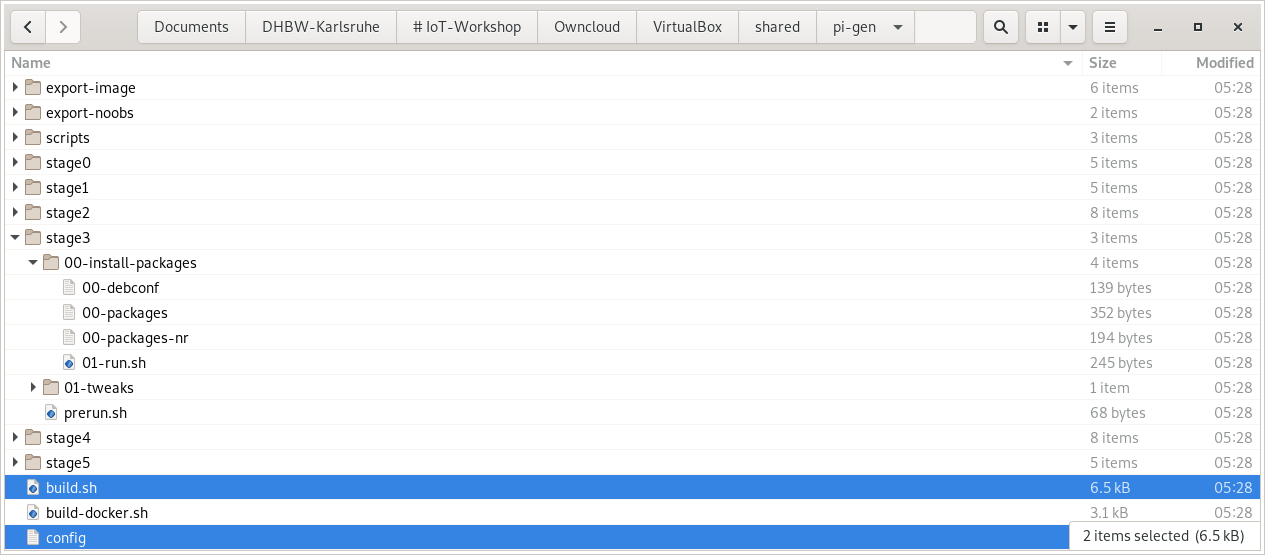
\includegraphics[width=\textwidth]{img/pi-gen-dateien}
    \vskip 1em

    {
        \footnotesize
        Konfiguration durch Anpassen und Ergänzen der Konfigurationsdateien und Shell-Skripte
    }

    \begin{columns}[T,onlytextwidth]
        \column{.5\textwidth}
        \begin{block}{Start des Build-Vorgangs}
            \texttt{./build.sh}
        \end{block}

        \column{.5\textwidth}
        \begin{block}{Durchschnittliche Laufzeit}
            \smallskip
            $\geq$ 30 Minuten konstant
        \end{block}
    \end{columns}
\end{frame}
}

%%% Folie
{
\small

\begin{frame}{Linux-Images bauen mit Buildroot}
        \href{https://buildroot.org/downloads/manual/manual.html}{\beamergotobutton{Offizielles Handbuch}}
        \href{https://www.wpvs.de/repo/iot-workshop/05-Werkzeuge/Erste\%20Schritte\%20mit\%20Linux,\%20Buildroot\%20und\%20Debootstrap.pdf}{\beamergotobutton{Vorlesungsskript}}

        \smallskip
        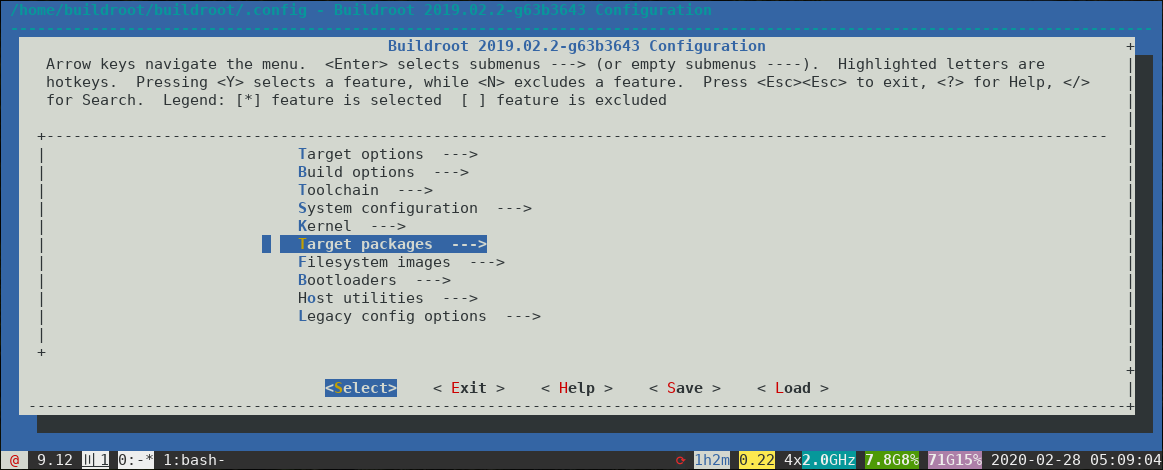
\includegraphics[width=\textwidth]{img/buildroot-menuconfig}
        \vskip 1em

        {
            \footnotesize
            \setlength{\tabcolsep}{0em}

            \begin{tabular}{p{.4\textwidth} p{.3\textwidth} p{.3\textwidth}}
                1. Vorlage laden &
                2. Konfiguration bearbeiten &
                3. Zusatzdateien bearbeiten \\

                \texttt{make raspberrypi3\_defconfig} &
                \texttt{make menuconfig} &
                \texttt{nano …} \\
            \end{tabular}
        }

    \begin{columns}[T,onlytextwidth]
        \column{.5\textwidth}
        \begin{block}{Start des Build-Vorgangs}
            \texttt{make BR2\_JLEVEL=4}
        \end{block}

        \column{.5\textwidth}
        \begin{block}{Durchschnittliche Laufzeit}
            \smallskip
            \parbox{\linewidth}{
                Mindestens eine Stunde beim ersten Durchlauf, wenige Minuten bei
                jedem Folgeaufruf
            }
        \end{block}
    \end{columns}
\end{frame}
}

% Fallbeispiel mit Python auf eigener Folie???

%%%% Folie
%\begin{frame}{Linux-Images bauen mit Ubuntu Core}
    %TODO
%\end{frame}

%%% Folie
\begin{frame}{Fazit und Ausblick}
    \begin{itemize}
        \justifying

        \item Linux eignet sich in besonderem Maße zur Entwicklung von IoT-
        und Embedded Devices aufgrund seines großen Funktionsumfangs und der
        enormen Flexibilität.

        \item Distributionen wie Raspbian bieten dabei auch für Einsteiger
        eine Möglichkeit, schnelle Erfolge zu erzielen.

        \item Für kleine Hobbyprojekte sowie Projekte mit wenigen Endgeräten
        reicht es häufig aus, einfach eine Standardinstallation von Rasbpian
        direkt auf dem Gerät an die eigenen Anforderungen anzupassen.

        \item In größeren Projekten ist es jedoch besser, das Betriebssystem als
        eigenständige Softwarekomponente zu betrachten, die wie jede Software
        mit geeigneten Werkzeugen \glqq{}entwickelt\grqq{} werden muss.

        \item Hierfür stehen verschiedene Baukästen zur Verfügung, welche die
        meisten Schritte dabei automatisieren.

        \item Leider besitzen die Baukasten-Systeme anfangs eine etwas hohe
        Einstiegshürde. Ist diese aber einmal genommen, lassen sich damit auf
        professionelle Art und Weise individualisierte Linux-Betriebssysteme bauen.
    \end{itemize}
\end{frame}

